\question{Cómo puedes determinar el valor de la resistencia al corte sin drenaje ($C_u$) de una arcilla a partir de un ensayo de compresión simple ? ¿ Qué fiabilidad te merece el resultado ?}{
	\begin{figure}[H]
			\centering
			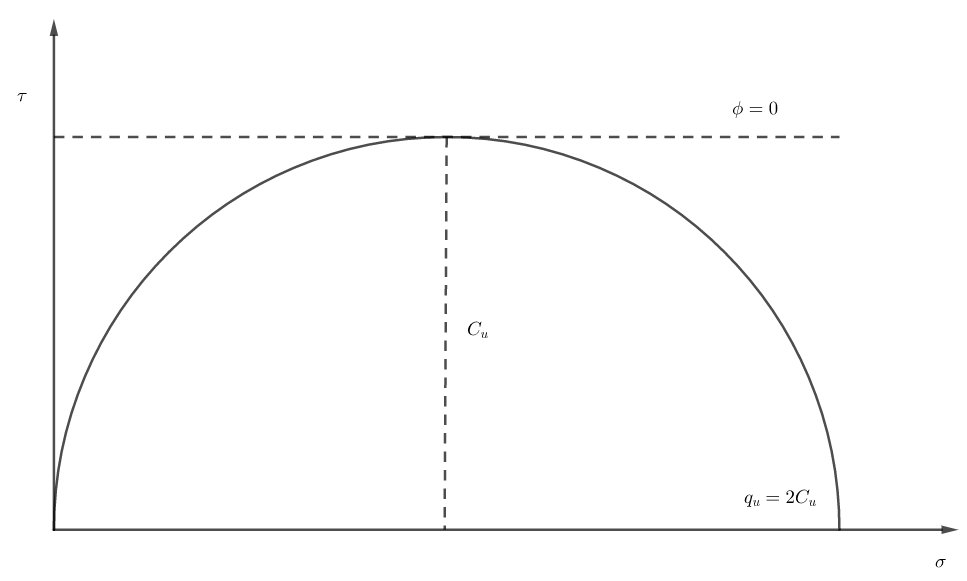
\includegraphics[width=0.5\textwidth]{img/cu}
			\caption{Circulo de Mohr: compresión simple sin drenaje}
			\label{fig:cu}
	\end{figure}
	Se rompen distintas provetas y se encuentra la envolvente de rotura. La fiabilidad del resultado dependerá del la alteración de la muestra.
}

\question{Cúando se utilizan los resultados del ensayo del molinete (vane-test) para estimar el valor de $C_u$ de una arcilla, se suele aplicar un factor de corrección que depende del índice de plasticidad del suelo. ¿ A qué se debe la necesidad de esta corrección? ¿ A partir de qué datos se ha determinado dicho factor?}{
	Se aplica por:
	\begin{itemize}
		\item Anisotropia del terreno
		\item Velocidad de cargo (más rapida que en campo)
	\end{itemize}
	Aplicamos un factor de corrección que varia en función del indice de plasticidad (IP), véase Figure~\ref{fig:mu}
	\begin{figure}[H]
			\centering
			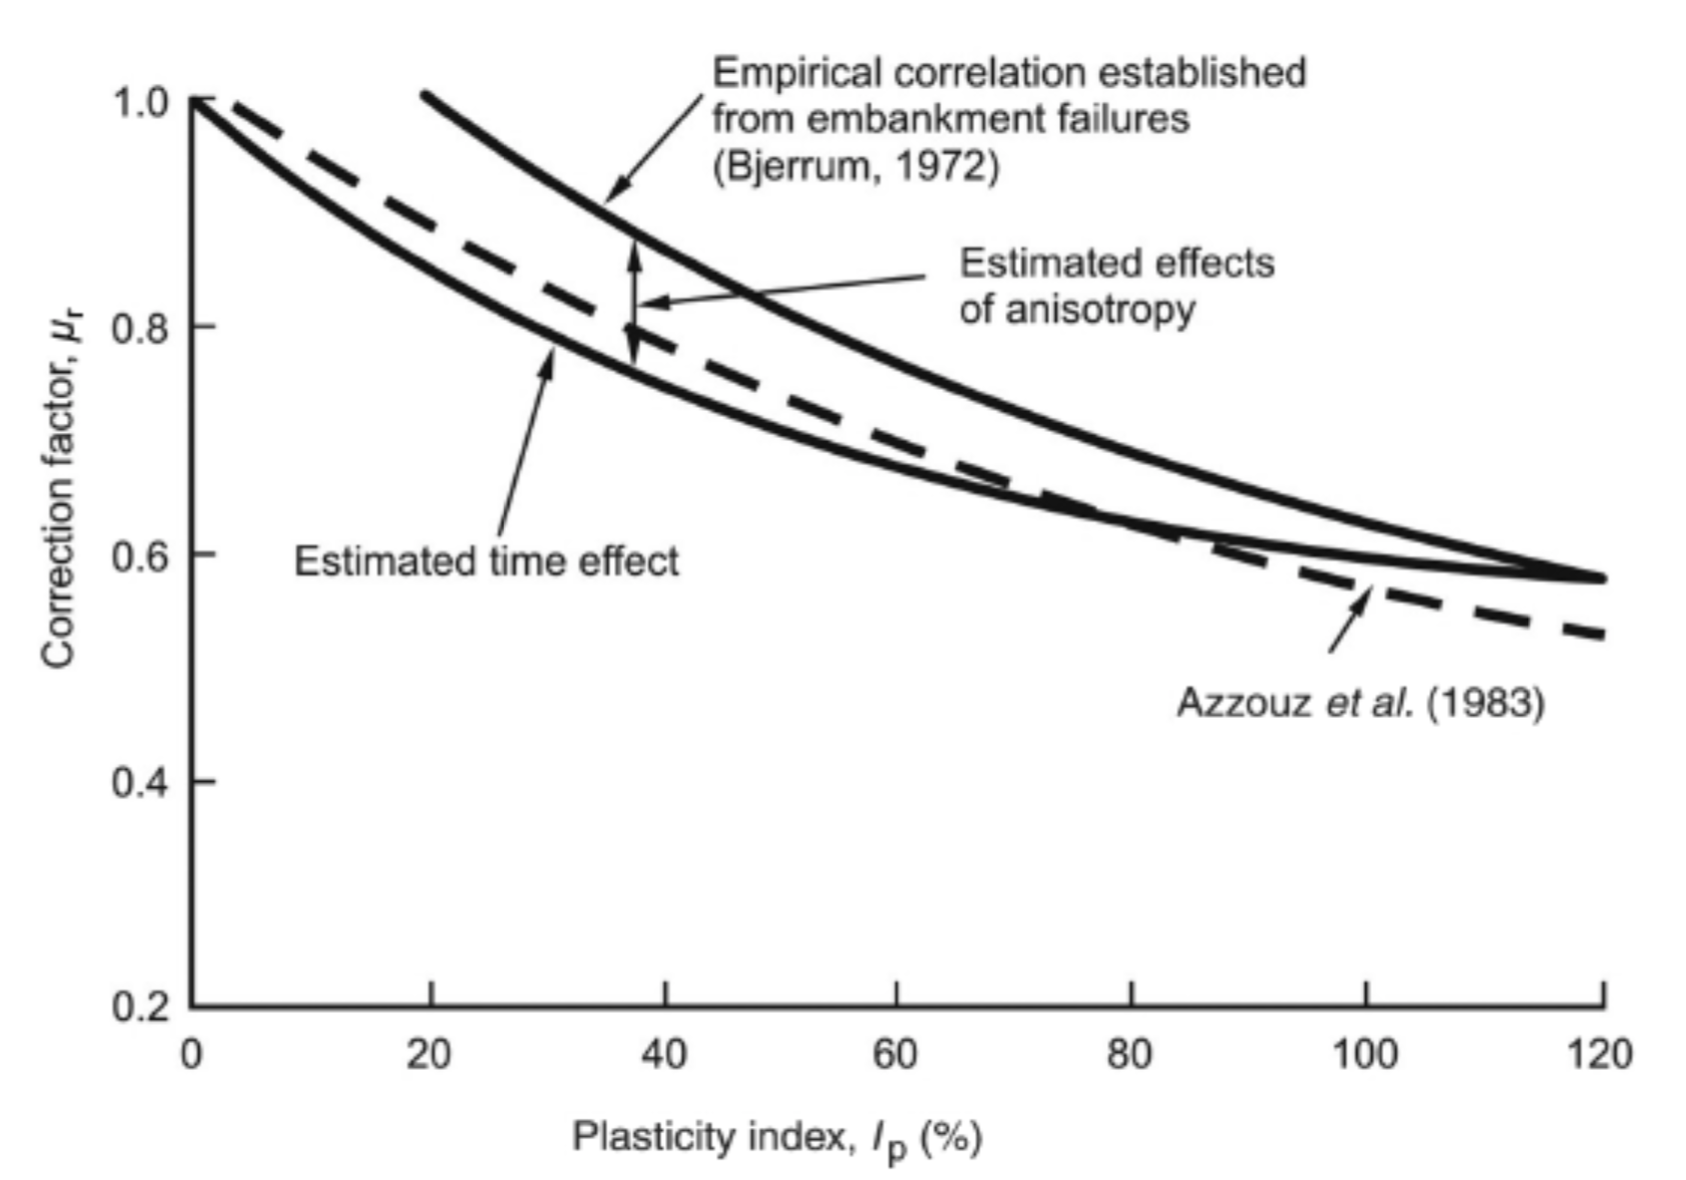
\includegraphics[width=0.5\textwidth]{img/mu}
			\caption{Factor de corrección Vane test}
			\label{fig:mu}
	\end{figure}
}

\question{Suponiendo que una arcilla se comporta con un modelo eláso-perfectamento plástico, dibujar la evolución de la presión intersticial que se medirá en un ensayo presiométrico (se considera condiciones no drenadas).}{
	\begin{figure}[H]
			\centering
			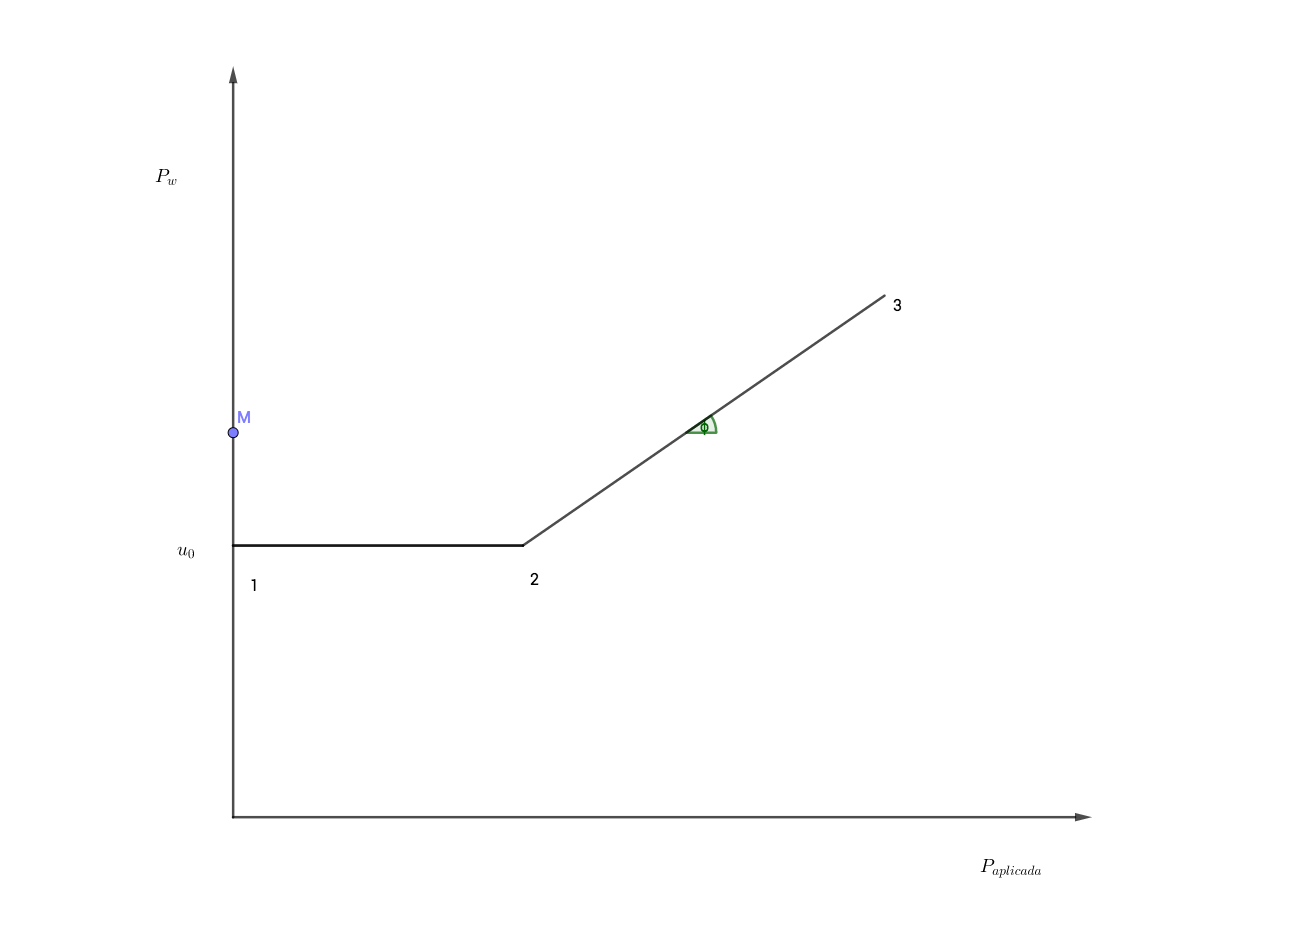
\includegraphics[width=0.5\textwidth]{img/u_evolution}
			\caption{Evolución de la presión intersticial}
			\label{fig:mu}
	\end{figure}
	Véase la evolución de los circulos de mohr en las Figure~\ref{fig:presio1},\ref{fig:presio2},\ref{fig:presio3}

	\begin{minipage}{0.5\linewidth}
		\begin{figure}[H]
		\centering
		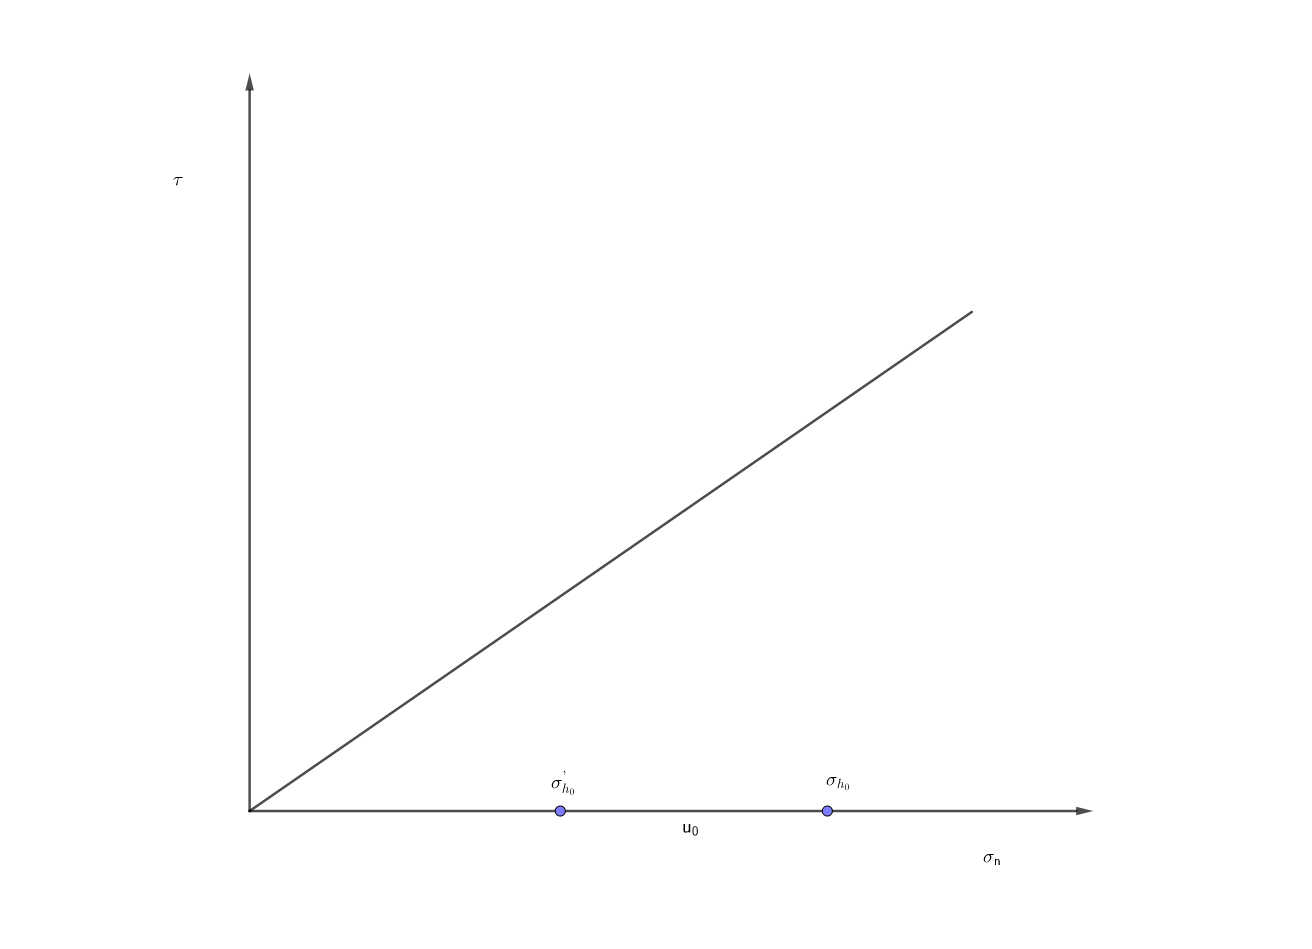
\includegraphics[width=\textwidth]{img/presio1}
		\caption{Estado inicial}
		\label{fig:presio1}
		\end{figure}
	\end{minipage}%
	\begin{minipage}{0.5\linewidth}
		\begin{figure}[H]
			\centering
			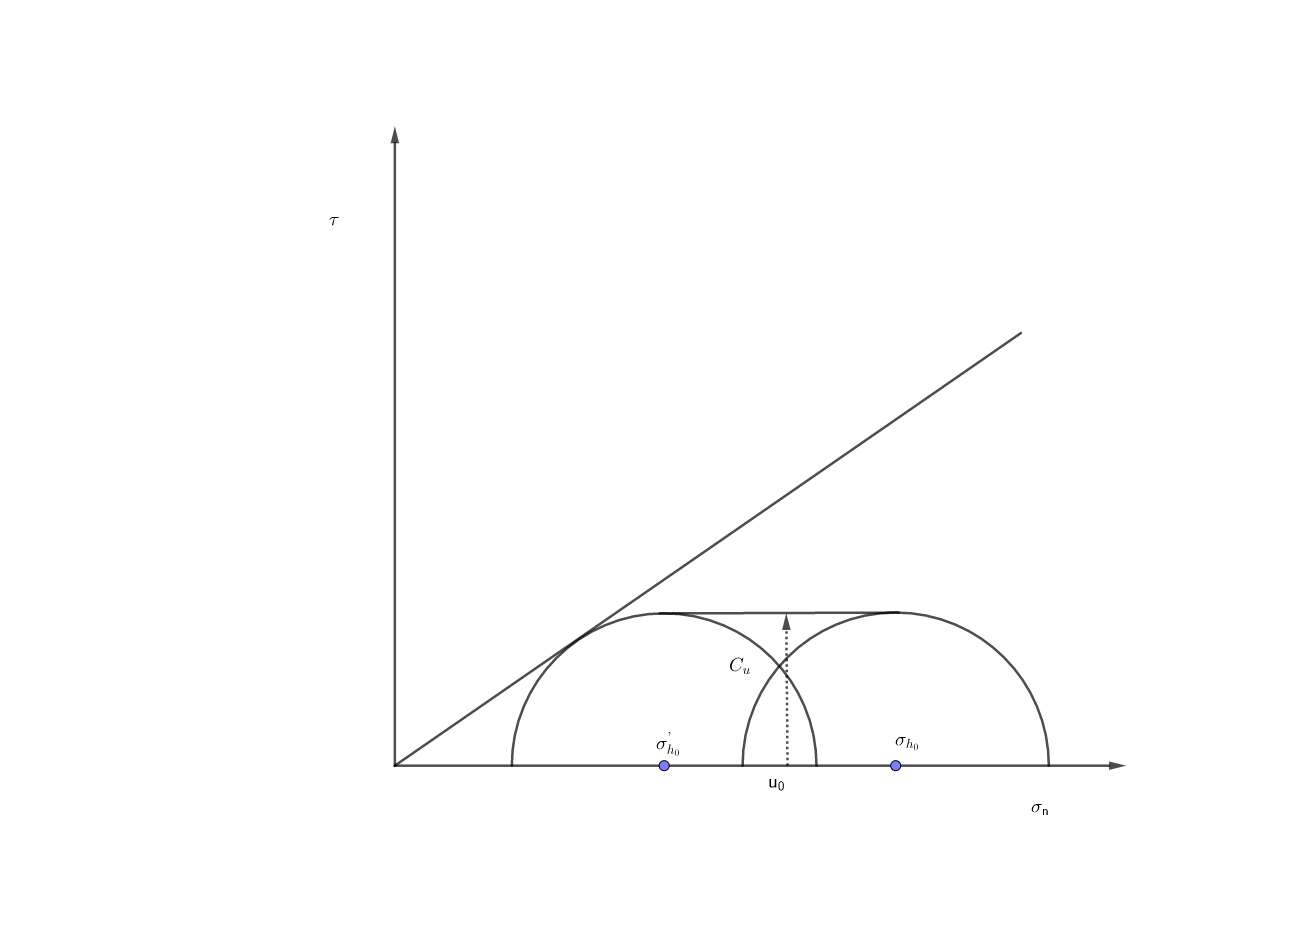
\includegraphics[width=\textwidth]{img/presio2}
			\caption{Incremento de presión con presión intersticial constante}
			\label{fig:presio2}
		\end{figure}
	\end{minipage}
	\begin{figure}[H]
			\centering
			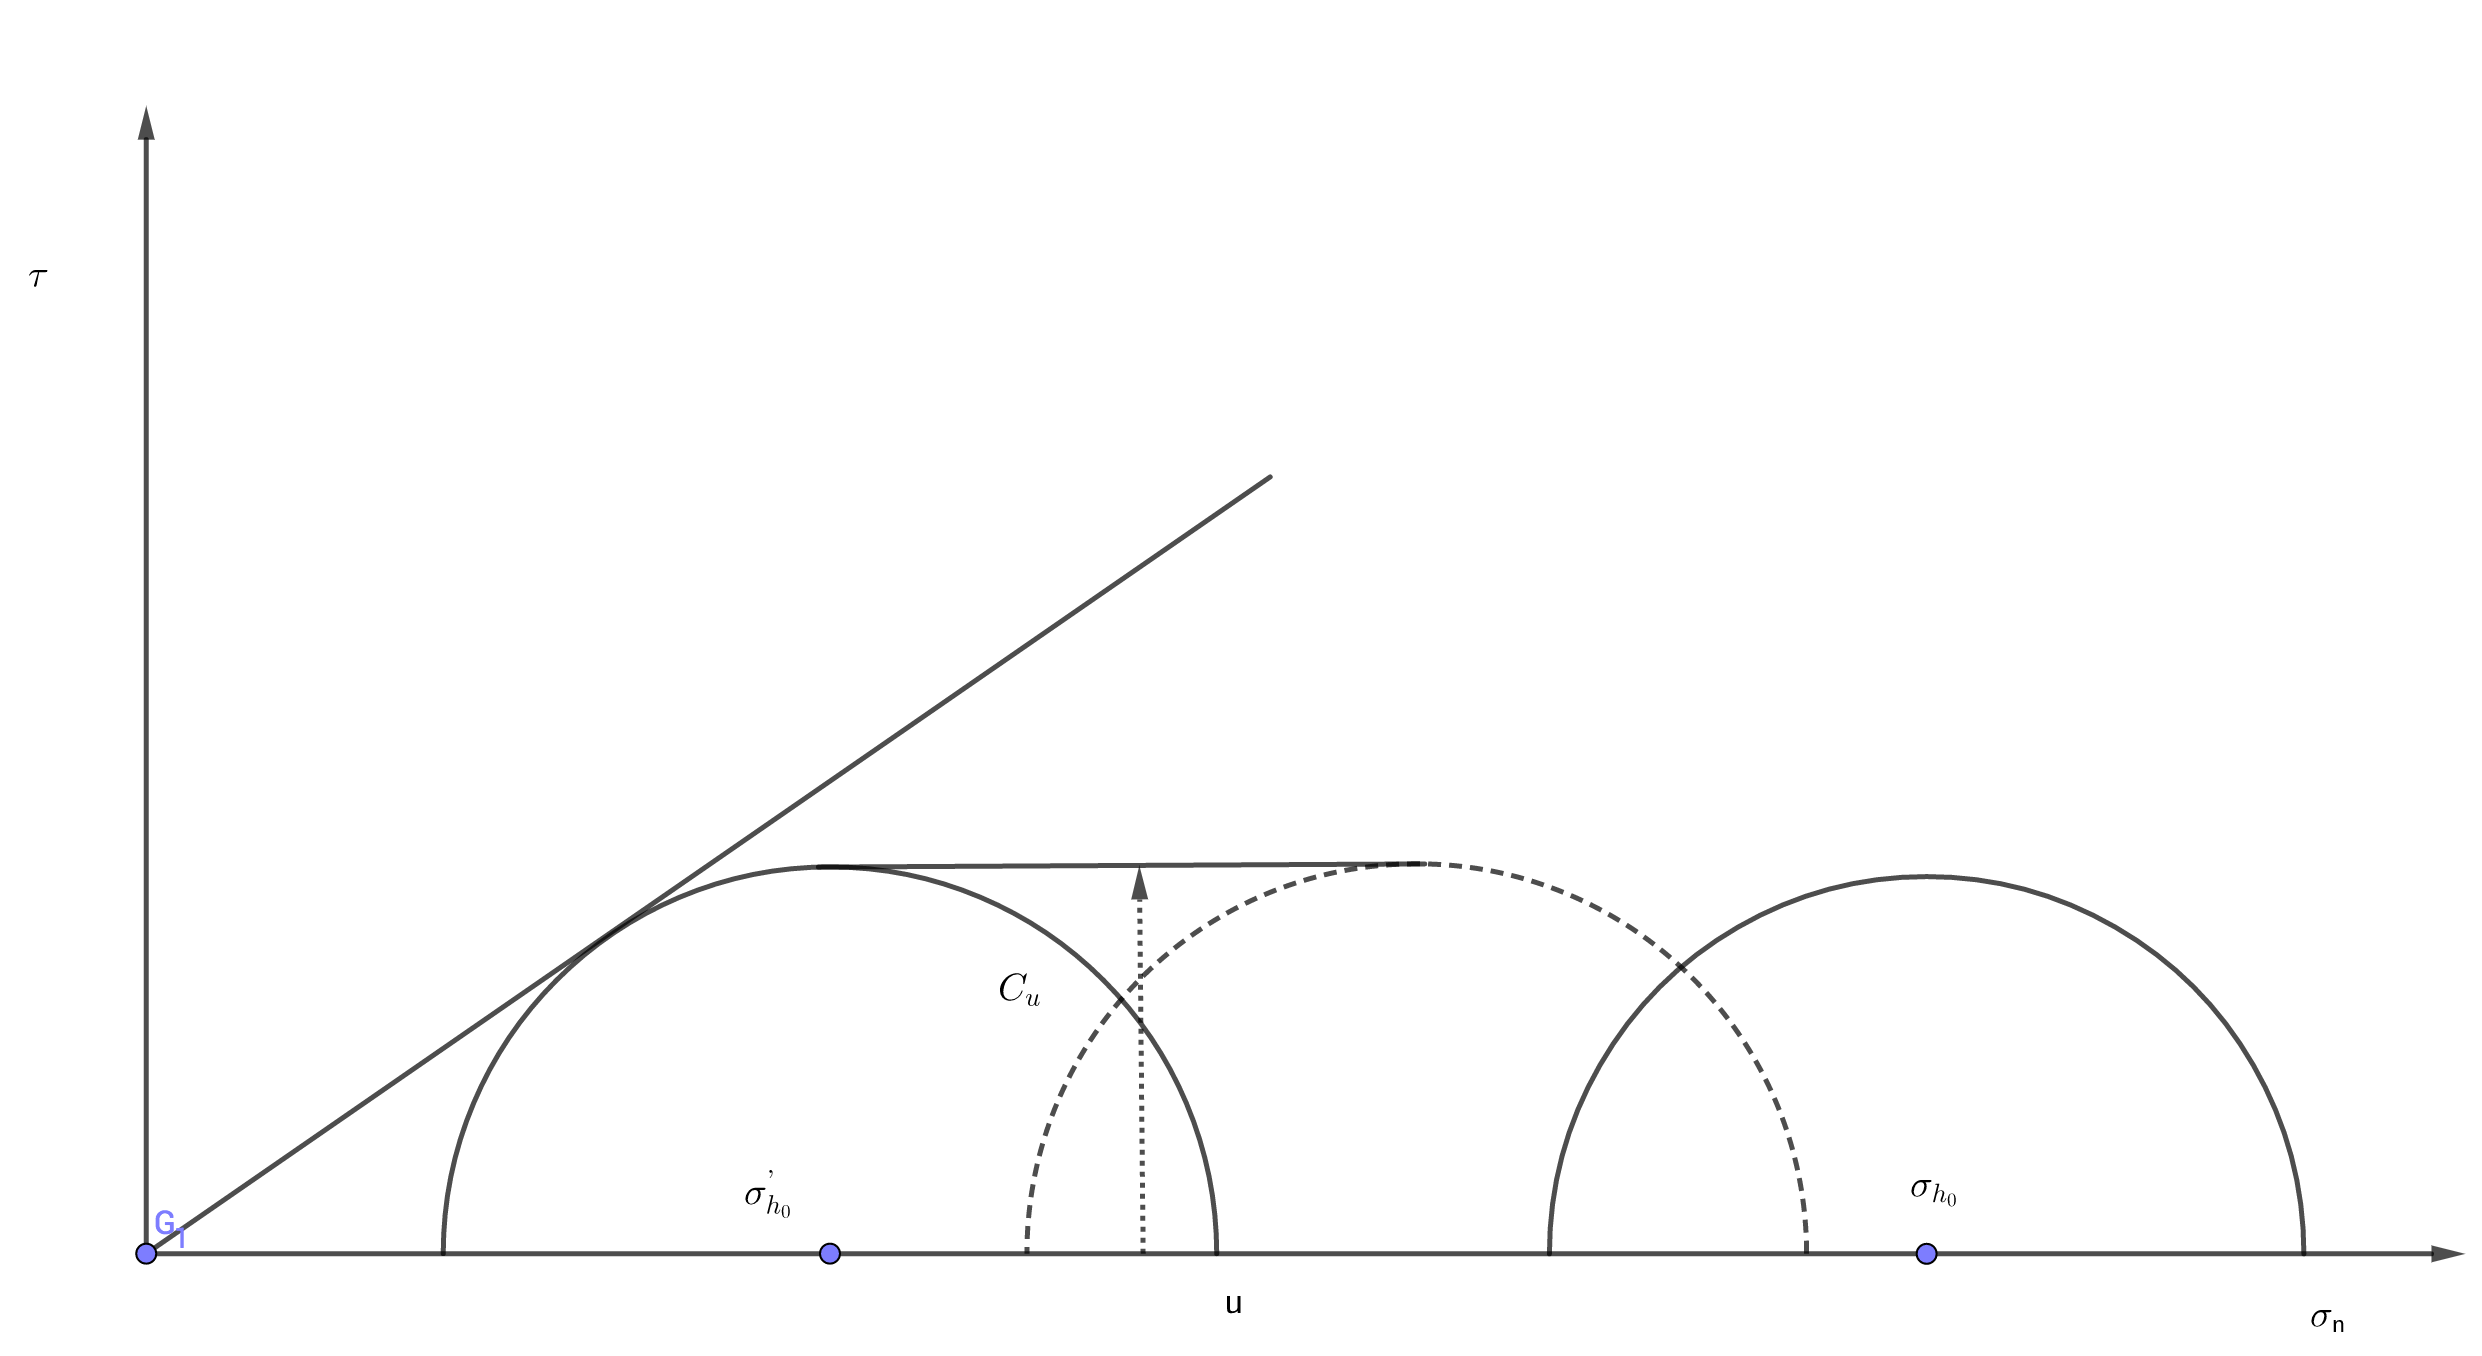
\includegraphics[width=0.6\textwidth]{img/presio3}
			\caption{Aumento de la presión intersticial}
			\label{fig:presio3}
	\end{figure}
}


% section questions (end)